\chapter{Software Heritage: the Great Library of Source Code}

\begin{figure}
    \centering
    
\includegraphics[width=0.5\linewidth]{img/SWH-logo}
    \caption{Logo of the Software Heritage initiative}
\end{figure}

\section{Project goals}

Launched in 2016, the Software Heritage
initiative\footnote{\url{https://www.softwareheritage.org/}}~\cite{swhcacm2018}
has the stated mission of collecting, preserving and sharing all the software
that is available in source code form, together with its entire development
history and associated metadata.

As software has become a key technology lying at the heart of our modern
civilization, it has become clear that it embodies a growing part of our shared
cultural, scientific and technical heritage, and as a result it has attracted
growing attention from the digital preservation community.
Recently, the focus of archival efforts have started to shift to preserve the
software \emph{source code}, which is where this technical knowledge is
embedded, rather than executable binaries which are mostly unreadable for
humans and stripped of all development insights. Developers sometimes tend to
call this source code the ``preferred form of modification'', emphasizing its
importance as the format that human programmers directly interact with when
writing software.

As a way to pursue this three-fold mission of collecting, preserving and
sharing the software commons, the Software Heritage initiative aims at becoming
three major things:

\begin{enumerate}
    \item A \textbf{reference catalog} of all the software source code. By
        painstakingly finding and referencing the extant source code and
        all the different places it appears in, the archive aims to become a
        general entry point where historical and contemporary software can be
        found and retrieved.
    \item A \textbf{universal archive} where the software is safely preserved
        in the long-term. There have been multiple occurrences of large troves
        of data being lost, be it for business-driven reasons (e.g., Gitorious,
        Google Code, Bitbucket), inconsiderate or malicious handling (e.g.,
        Code Spaces) or gradual data degradation over time, which have
        highlighted the need for an infrastructure to protect these commons.
    \item A \textbf{research platform} to enable analysis of all the source
        code in the archive. This implies making the data not only
        \emph{available}, but also \emph{accessible} to researchers and
        industrials, by providing a framework to perform experiments in ways
        that are convenient and suitable for large-scale data mining.
\end{enumerate}

The work presented in this thesis is focused on the latter point and explores
various directions to enable large-scale analysis of the software source code
present in the archive. However, to understand \emph{how} we intend to make
this data accessible, we first have to look at the way the archive works: its
scale, what it covers, how its data is crawled and ingested, how the archive
grows over time, etc.

\section{Software collection}

\subsection{Finding all the source code}

While the Software Heritage archive aims to assemble and preserve \emph{all}
the software source code, all software projects are not equal in terms of ease of
collection. \figref{fig:swh-collect-axes} shows how this complexity can be
mapped on two axes. The Open $\leftrightarrow$ Closed axis references the right
to archive the source code, as obtaining the right to archive private
repositories is more challenging than for ones already open to the public.  The
Online $\leftrightarrow$ Offline axis indicates whether the software is already
online in a digital format on a (potentially private) network, or whether it
would require efforts to retrieve it from a physical medium, such as offline
hard drives or even old source listings.

Each quadrant will entail different resources and techniques to be ingested in
the archive. Naturally, the Software Heritage initiative has thus far focused
its resources predominantly on the top-right quadrant, i.e., source code that is
already publicly available online on code hosting platforms, due to how
comparatively easy it is to automate the retrieval of large quantities of
software source code.  Throughout this thesis, we focus on what we call
\emph{public development}, which mainly refers to this quadrant of open and
online software.

Note that this has implications for empirical research: knowledge gained from
studies on the data amassed by Software Heritage will necessarily have a
selection bias, as it will capture the patterns that are specifically
found in public development. A general rule is that the more accessible a
piece of source code already is (by being present on well-known hosting
platforms), the more likely it is to be archived in Software Heritage.

\begin{figure}
    \centering
    \begin{tikzpicture}
        \node [above] at (5,0)  {\textbf{Open}};
        \node [above] at (-5,0) {\textbf{Closed}};
        \node [right] at (0,3)  {\textbf{Online}};
        \node [right] at (0,-3) {\textbf{Offline}};
        \draw [<->] (0,-3) -- (0,3);
        \draw [<->] (-5,0) -- (5,0);

        \node [align=left] at (2.5,1.5) {Automation};
        \node [align=left] at (2.5,-1.5) {Crowdsourcing};
        \node [align=left] at (-2.5,-1.5) {Focused search};
        \node [align=left] at (-2.5,1.5) {Escrow};
    \end{tikzpicture}
    % 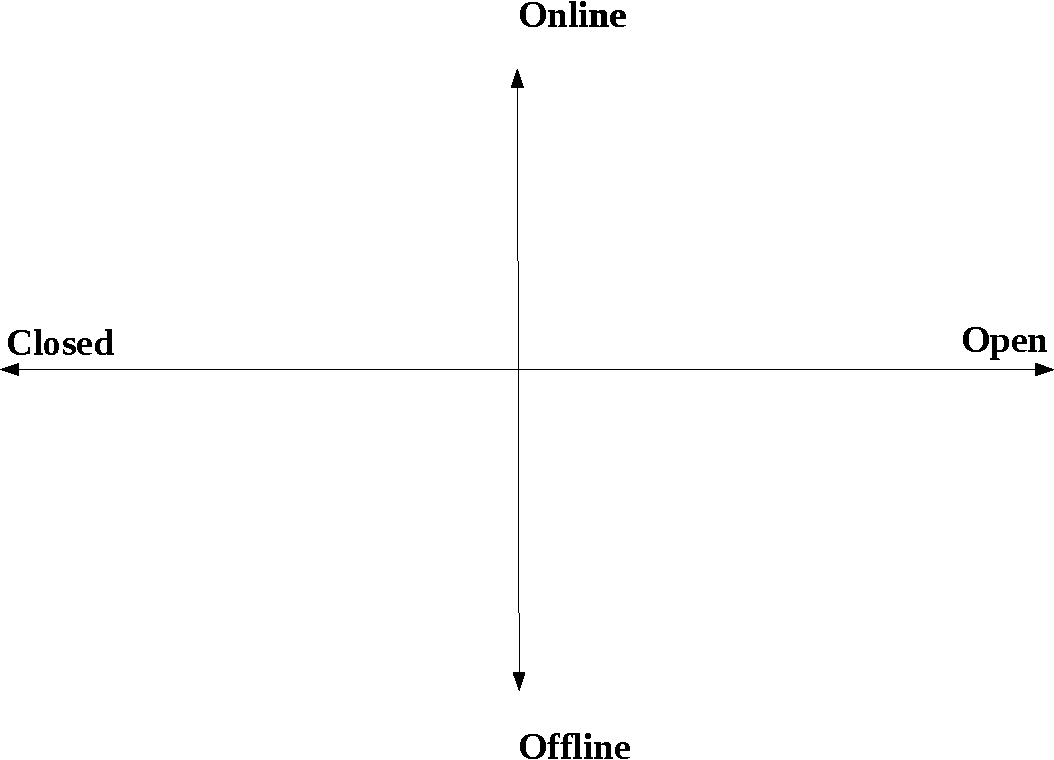
\includegraphics[width=0.5\linewidth]{img/swh-collect-axes}
    \caption{Two axes of software collection, with each quadrant its
    retrieval challenges}%
    \label{fig:swh-collect-axes}
\end{figure}

\subsection{Software origins}

\emph{Software origins} are abstract objects representing the places where we
can find a given piece of software source code. In practice, they are often
represented in the form of a URL, pointing to the web page where a given
software was found.

Origins are conceptually different from \emph{projects}. A specific software
project can be found in multiple origins, especially in the case of \glspl{DVCS}
where there is no central authority to be the main place of development of the
software. As an example, Linus Torvalds' version of the Linux repository is
hosted in at least three different origins:

\begin{itemize}[ ]
    \setlength\itemsep{-0.5em}
    \item \url{https://github.com/torvalds/linux}
    \item \url{https://git.kernel.org/pub/scm/linux/kernel/git/torvalds/linux.git}
    \item \url{https://gitlab.com/linux-kernel/linux}
\end{itemize}

Additionally, developers using \glspl{DVCS} can upload their own working copy of
the repository they are working on, thereby creating more origins of the same
software. Greg Kroah-Hartman has his own working copy of the Linux repository
hosted at \url{https://github.com/gregkh/linux}. All in all, there can be
thousands of origins hosted in different places, all pointing to the same
software source code.

Origins are often found in code hosting platforms called \emph{software
forges}~\cite{squire2012describing, DBLP:conf/wikis/Squire17}. These forges are
hubs for software development, aggregating and organizing code repositories as
well as their associated project metadata like issues, bug reports, continuous
integration services, etc.  These forges can be centralized services where any
developer is free to upload their own repository. GitHub is by far the largest
example of such a centralized platform, totaling 40 million users and more than
190 million repositories as of January 2020. Other forges like GitLab or
Phabricator function on a more decentralized model, where the code of the forge
itself is open source, and organizations can self-host their own instances of
the forge to store and organize their projects.

Another source of origins is curated software ecosystems, like app stores or
package manager repositories~\cite{DBLP:conf/msr/KikasGDP17,
DBLP:conf/msr/AbateCGFTZ15}. For instance, Linux distributions like Debian
generally maintain a set of software packages that are published online, and
users can use the package manager of their distribution to automatically
install or upgrade the software in their operating system. Programming language
ecosystems also often have their own package managers as a way for developers
to quickly install libraries and frameworks that their own software depends on,
for instance the Python language uses the PyPI repository, and Javascript uses
the NPM registry.

\subsection{Archival process}

Indexing every single software origin that exists in order to ingest them in
the archive would be an incredibly tedious task. Fortunately, this process can
largely be automated with the use of \emph{listers}. Over the years, Software
Heritage has been continuously establishing a list of software forges and
package repositories where publicly available software can be retrieved and
archived. Generally, these code hosting platforms provide APIs that can be used
to get a list of all the projects hosted on the platform. The Software Heritage
listers use these APIs to periodically get a list of all the repositories in
the forge and schedule them to be loaded in the archive. Some forges also
support subscribing to event feeds when repositories get added or modified,
which is used to schedule repositories at a finer granularity.

Of course, the software found when visiting an origin can be stored under a
variety of formats: a source code repository can be versioned under one of the
many \glspl{VCS} in existence (Git, Mercurial, SVN, Bazaar, etc.), or even just
released as a succession of tarball archives. Likewise, package managers all
have specific packaging formats that they use to track package metadata and
installation rules (e.g., deb and RPM files).

The role of understanding and processing the various formats of code
repositories to archive is delegated to another component in the Software
Heritage infrastructure, the \emph{loaders}. Each loader is written for a
specific type of \gls{VCS} repository or source package, and thus all the
formats supported by the Software Heritage archive have their own loader. To
ingest a code repository in the archive, the loaders first retrieve it from the
remote either by communicating in the protocol of the VCS, or using a simple
downloading protocol like HTTP, FTP or rsync. Then, they extract all the
different software artifacts contained in the repository and ingest them in the
archive.

\begin{figure}
\begin{center}
    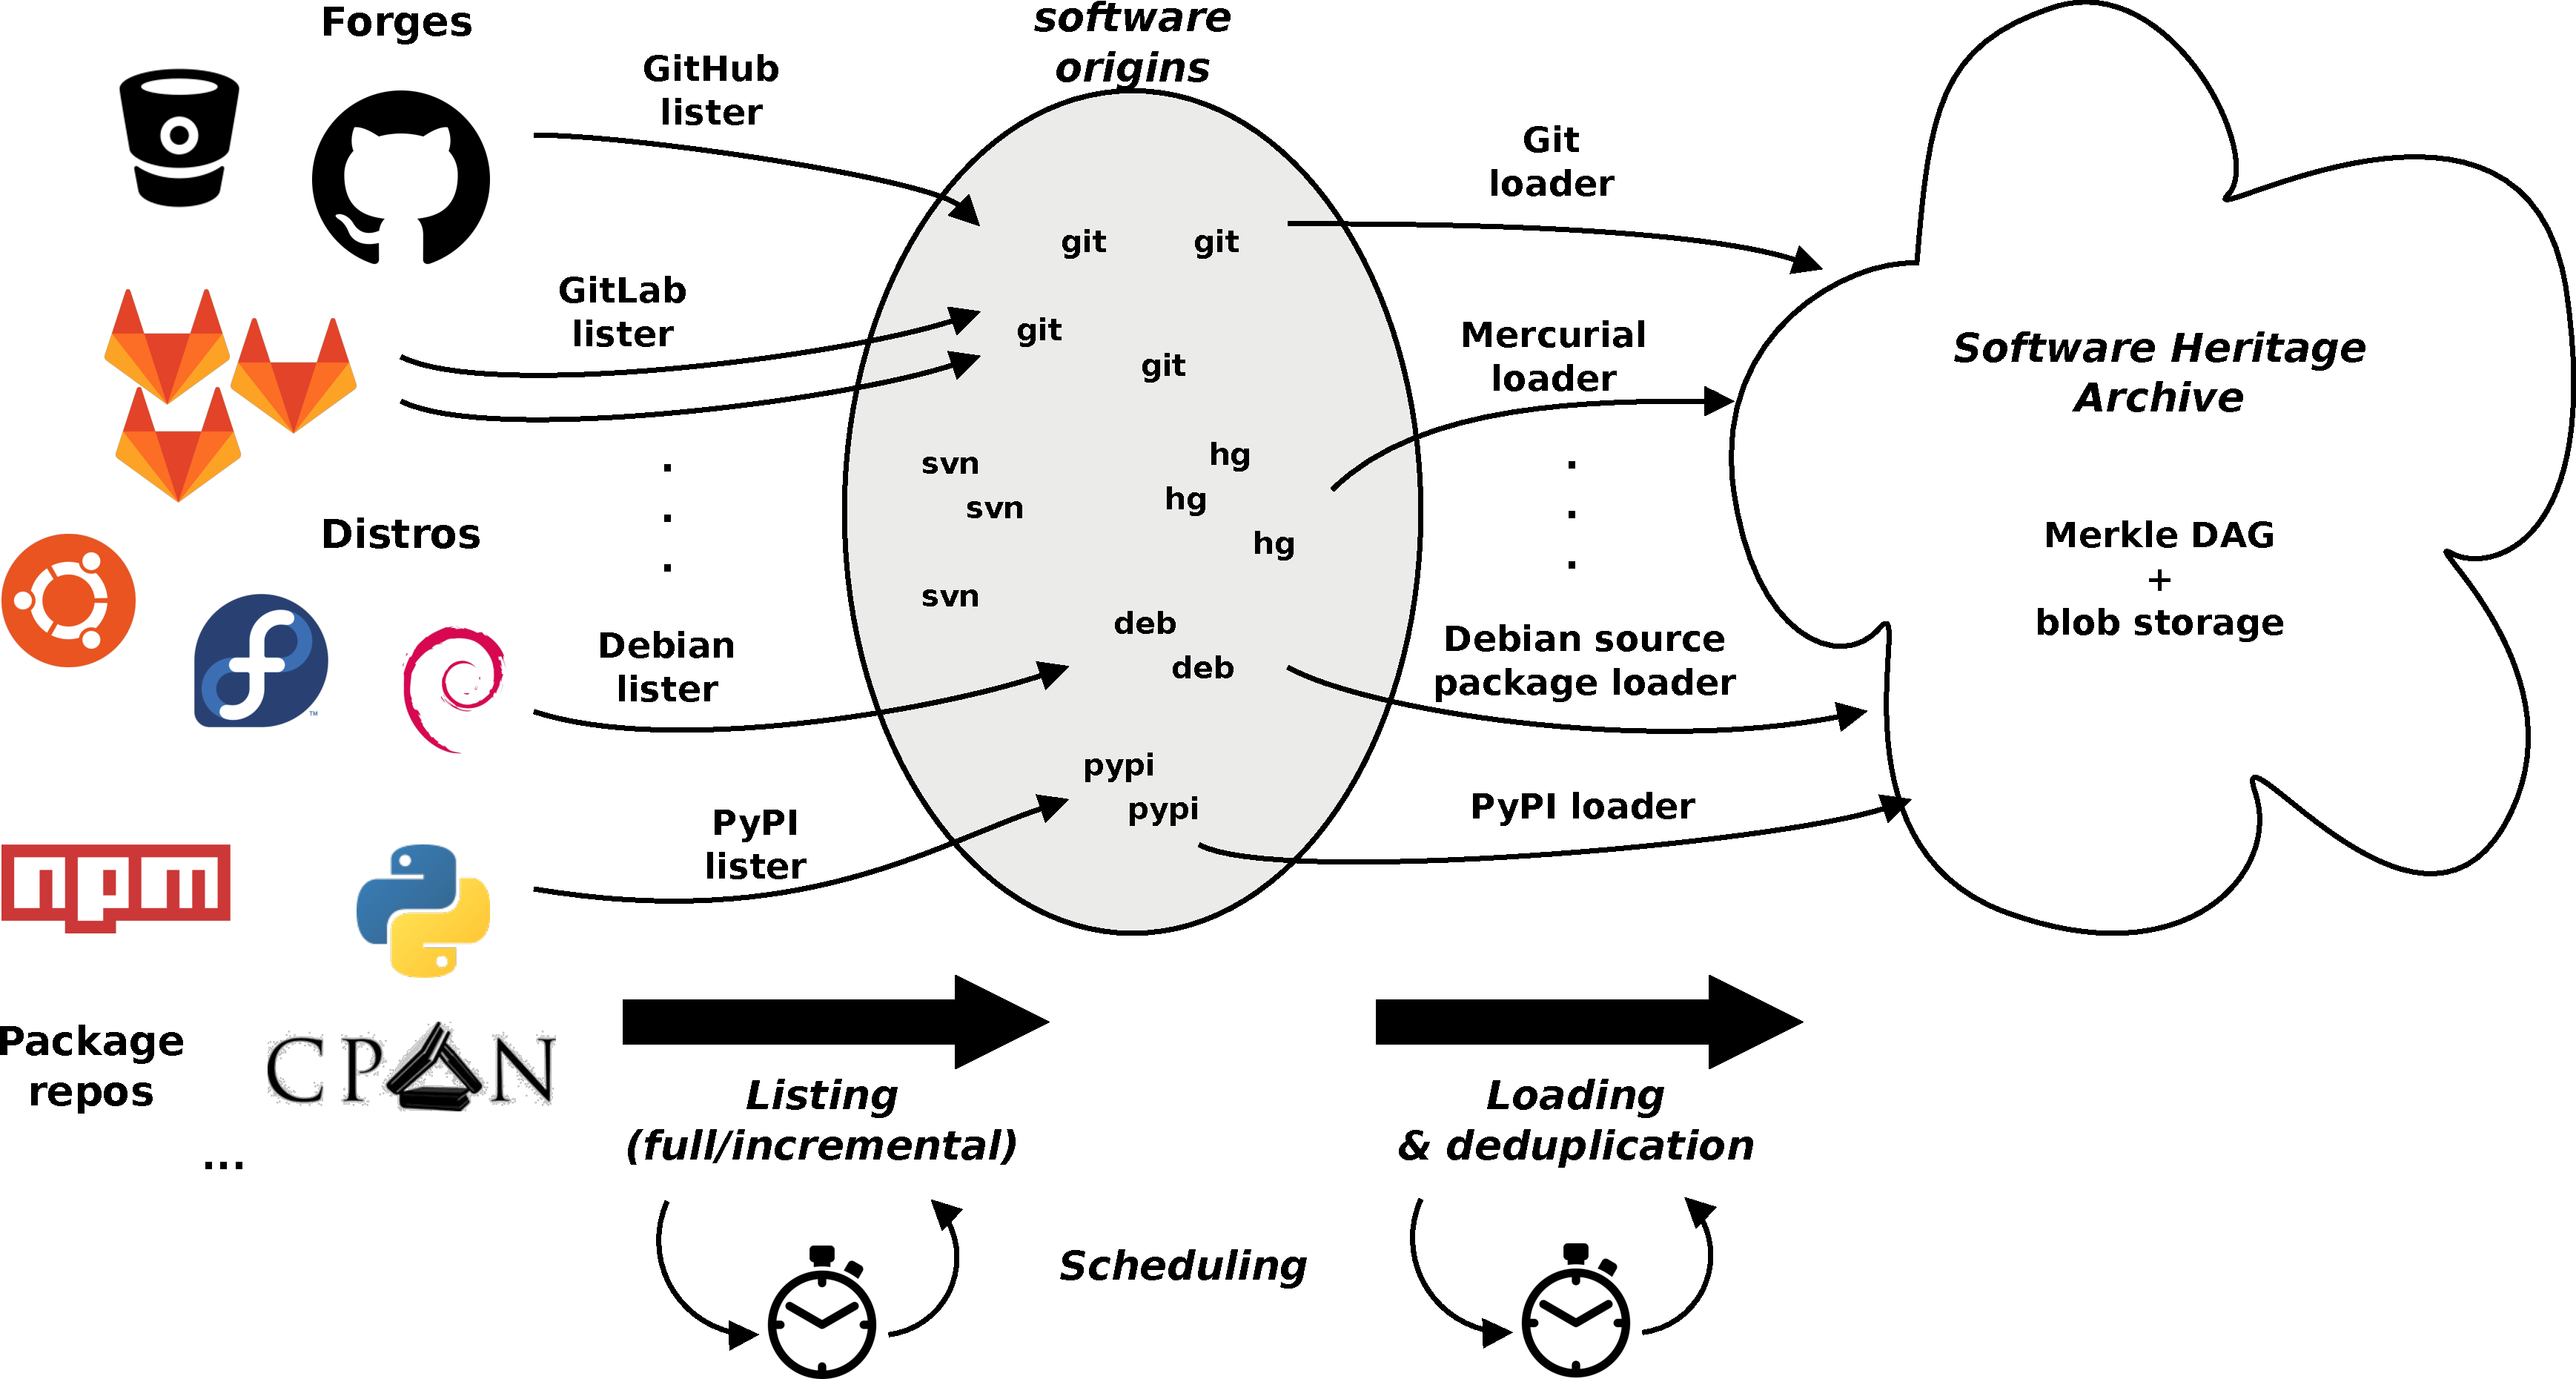
\includegraphics[width=0.9\textwidth]{img/swh-dataflow}
\end{center}
\caption{Data flow of the archival process}%
\label{fig:archival-data-flow}
\end{figure}

This entire archival process is shown in~\figref{fig:archival-data-flow}. One
important thing to note is that while the input projects are all retrieved in
very heterogenous formats, the loaders do not keep the data that way: they
transform the artifacts in a \emph{canonical format} that allows the entire
archive to be a unified and deduplicated collection of software artifacts,
thanks to a comprehensive data model described in Chapter~\ref{chp:swh-model}.

\subsection{Software notability}

One of the stated goals of the Software Heritage initative is exhaustiveness,
which implies not making value judgments as to what constitutes ``important''
or ``notable'' software. At no point in this process does any filtering occur
that would remove software artifacts considered unimportant or irrelevant:
binary files, unpopular projects, source file in unknown languages etc.\ are
all ingested as first-class citizens in the archive. The only limits enforced
are technical limitations and those that help prevent abuse: software artifacts
larger than a few hundred megabytes are considered to be outside of the scope
of the archive and are not inserted in it.

A rationale for that design choice is that there is no way to know \emph{a
priori} which software is going to be notable in the future, as most software
projects start small then gain popularity over time. By the time a project
would have reached notability threshold, traces of its past history could have
already been lost. This exhaustiveness principle allows us to follow in real
time the evolution and growth of projects and the social processes that govern
their communities.

One side effect of this design is that the archive contains a lot of data that
is not typically considered to be software source code: homepages, datasets,
configuration files, periodical database dumps, images and other assets, etc.
While software forges are mostly used as a source code development platform,
they can also be used as general hosting providers in some cases. Researchers
should be aware of this fact when exploiting the data in the archive, and
filter out these non-source code objects if desired.

% Scope?
\section{The world's largest repository of source code}

\subsection{Coverage}

Software Heritage has a coverage from a wide array of sources thanks to its
numerous listers and loaders and its extensible framework for adding new data
sources. The loaders are capable of processing and ingesting the three most
popular \glspl{VCS} currently in use: Git, Mercurial and SVN\@. They also handle
the packages of the Linux distributions Debian, Nix and Guix, as well as those
from the repositories PyPI, CRAN, NPM and Packagist (respectively for the
Python, R, Javascript and PHP programming languages).

The listers are configured to run on the major code hosting platforms, and the
archive contains a full copy of GitHub, Bitbucket, GitLab, SourceForge and the
GNU project. They also periodically crawl the repositories of hundreds of
decentralized instances of Phabricator, GitLab, cgit, Launchpad and Gitea.
Some of the projects preserved in the archive were also recovered from defunct
hosting platforms such as Gitorious and Google Code, then loaded as a one-shot
task, as those sources do not require recurrent listing.

\TODO{More fine-grained breakdown of the archive content by forge, like a table
or a piechart. Take the one from the topology article?}

This extensive and far-reaching coverage has implications for research, as it
allows us to identify heterogenous properties that appear when doing analysis
across different \glspl{VCS} used on different hosting platforms. Finding
patterns and training models on the Software Heritage archive can be a way to
ensure robustness and applicability to a diverse mosaic of collaboration and
development practices.

\subsection{Current scale and future growth}

\begin{figure}
    \centering
    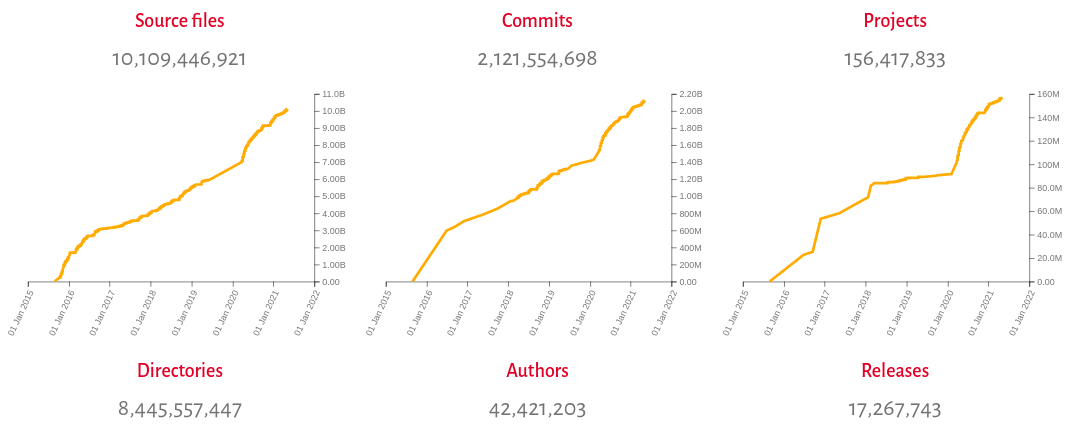
\includegraphics[width=0.9\linewidth]{img/swh-size}
    \caption{Size of the Software Heritage archive as of May 3, 2021}%
    \label{fig:swh-size}
\end{figure}

As of May 2021, the archive has ingested more than 10 billion source files from
156 million software origins. In the \gls{VCS} history, we identified as many
as 42 million different authors of more than 2.1 billion commits.
\figref{fig:swh-size} shows the growth of the archive over time in terms of the
number of source files, commits and projects stored.

Together, these source code files would weigh around 850\,TiB in total.
However, they are compressed in the main in-house storage, which reduces their
on-disk size to around half of that.\TODO{more precise number?} While the
source code files themselves take a huge amount of space, the other software
artifacts (directory trees, development history checkpoints, origins, etc.)
weigh significantly less overall. They are stored in a PostgreSQL database
which weighs around 7\,TiB in total, including database indexes on some fields
to allow for more efficient retrieval operations.

The archive is expected to grow over time as more and more listers,
loaders and data sources are added to the crawling process, but maybe more
importantly because of the natural growth rate of the quantity of code produced
worldwide over the years. In~\cite{swh-provenance-emse}, Rousseau, Di Cosmo and
Zacchiroli project this growth using the commit timestamps over a period of
more than 40 years, and find that the amount of commits in public source code
doubles every $\approx 30$ months, while the number of unique source code files
doubles every $\approx 22$ months. Zacchiroli further
confirmed~\cite{ieee-sw-gender-swh} this exponential trend while studying
historical gender differences in public software development. As of current
projections, this exponential growth is still assumed to be sustainable at the
scale of the archival project due to the also exponentially decreasing cost of
storage~\cite{swh-provenance-emse}.

The massive scale of the archive as well as its projected growth in the
foreseeable future highlights the architectural need for large scale
infrastructures to collect, store, analyze and make the data accessible to
researchers. This has a key implication taken into account throughout this
thesis, that designs of research platforms should precautiously take that
growth into account and aim to be as scalable as possible to be sustainable in
the long term.

\begin{figure}
    \centering
    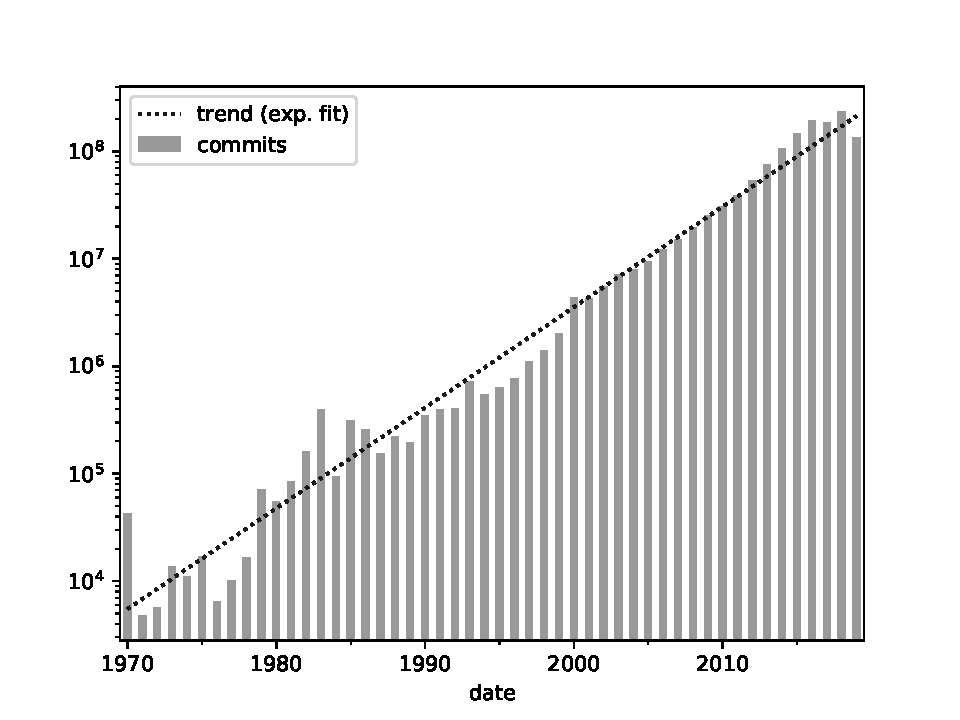
\includegraphics[width=0.5\linewidth]{img/commit-growth}
    \caption{Total number of yearly commits, increasing
    exponentially~\cite{ieee-sw-gender-swh}}%
    \label{fig:swh-commit-growth}
\end{figure}
